\documentclass[10pt]{foi}
\def\UrlBreaks{\do\/\do-}

\usepackage[breakable]{tcolorbox}
%\usepackage{parskip} % Stop auto-indenting (to mimic markdown behaviour)

%\usepackage[utf-8]{inputenc}
\usepackage{iftex}
\ifPDFTeX
\usepackage[T1]{fontenc}
\usepackage{mathpazo}
\else
\usepackage{fontspec}
\fi

% Basic figure setup, for now with no caption control since it's done
% automatically by Pandoc (which extracts ![](path) syntax from Markdown).
\usepackage{graphicx}
% Maintain compatibility with old templates. Remove in nbconvert 6.0
\let\Oldincludegraphics\includegraphics
% Ensure that by default, figures have no caption (until we provide a
% proper Figure object with a Caption API and a way to capture that
% in the conversion process - todo).
\usepackage{caption}
% \DeclareCaptionFormat{nocaption}{}
% \captionsetup{format=nocaption,aboveskip=0pt,belowskip=0pt}

\usepackage[Export]{adjustbox} % Used to constrain images to a maximum size
\adjustboxset{max size={0.9\linewidth}{0.9\paperheight}}
\usepackage{float}
\floatplacement{figure}{H} % forces figures to be placed at the correct location
\usepackage{xcolor} % Allow colors to be defined
\usepackage{enumerate} % Needed for markdown enumerations to work
\usepackage{geometry} % Used to adjust the document margins
\usepackage{amsmath} % Equations
\usepackage{amssymb} % Equations
\usepackage{textcomp} % defines textquotesingle
% Hack from http://tex.stackexchange.com/a/47451/13684:
\AtBeginDocument{%
\def\PYZsq{\textquotesingle}% Upright quotes in Pygmentized code
}
\usepackage{upquote} % Upright quotes for verbatim code
\usepackage{eurosym} % defines \euro
\usepackage[mathletters]{ucs} % Extended unicode (utf-8) support
\usepackage{fancyvrb} % verbatim replacement that allows latex
\usepackage{grffile} % extends the file name processing of package graphics
		 % to support a larger range
\makeatletter % fix for grffile with XeLaTeX
\def\Gread@@xetex#1{%
\IfFileExists{"\Gin@base".bb}%
{\Gread@eps{\Gin@base.bb}}%
{\Gread@@xetex@aux#1}%
}
\makeatother

% The hyperref package gives us a pdf with properly built
% internal navigation ('pdf bookmarks' for the table of contents,
% internal cross-reference links, web links for URLs, etc.)
\usepackage{hyperref}
% The default LaTeX title has an obnoxious amount of whitespace. By default,
% titling removes some of it. It also provides customization options.
%\usepackage{titling}
\usepackage{longtable} % longtable support required by pandoc >1.10
\usepackage{booktabs}  % table support for pandoc > 1.12.2
%\usepackage[inline]{enumitem} % IRkernel/repr support (it uses the enumerate* environment)
%\usepackage[normalem]{ulem} % ulem is needed to support strikethroughs (\sout) normalem makes italics be italics, not underlines
%\usepackage{mathrsfs}
% Colors for the hyperref package
\definecolor{urlcolor}{rgb}{0,.145,.698}
\definecolor{linkcolor}{rgb}{0,0.0}
\definecolor{citecolor}{rgb}{.12,.54,.11}

% ANSI colors
\definecolor{ansi-black}{HTML}{3E424D}
\definecolor{ansi-black-intense}{HTML}{282C36}
\definecolor{ansi-red}{HTML}{E75C58}
\definecolor{ansi-red-intense}{HTML}{B22B31}
\definecolor{ansi-green}{HTML}{00A250}
\definecolor{ansi-green-intense}{HTML}{007427}
\definecolor{ansi-yellow}{HTML}{DDB62B}
\definecolor{ansi-yellow-intense}{HTML}{B27D12}
\definecolor{ansi-blue}{HTML}{208FFB}
\definecolor{ansi-blue-intense}{HTML}{0065CA}
\definecolor{ansi-magenta}{HTML}{D160C4}
\definecolor{ansi-magenta-intense}{HTML}{A03196}
\definecolor{ansi-cyan}{HTML}{60C6C8}
\definecolor{ansi-cyan-intense}{HTML}{258F8F}
\definecolor{ansi-white}{HTML}{C5C1B4}
\definecolor{ansi-white-intense}{HTML}{A1A6B2}
\definecolor{ansi-default-inverse-fg}{HTML}{FFFFFF}
\definecolor{ansi-default-inverse-bg}{HTML}{000000}

% commands and environments needed by pandoc snippets
% extracted from the output of `pandoc -s`
\providecommand{\tightlist}{%
\setlength{\itemsep}{0pt}\setlength{\parskip}{0pt}}
\DefineVerbatimEnvironment{Highlighting}{Verbatim}{commandchars=\\\{\}}
% Add ',fontsize=\small' for more characters per line
\newenvironment{Shaded}{}{}
\newcommand{\KeywordTok}[1]{\textcolor[rgb]{0.00,0.44,0.13}{\textbf{{#1}}}}
\newcommand{\DataTypeTok}[1]{\textcolor[rgb]{0.56,0.13,0.00}{{#1}}}
\newcommand{\DecValTok}[1]{\textcolor[rgb]{0.25,0.63,0.44}{{#1}}}
\newcommand{\BaseNTok}[1]{\textcolor[rgb]{0.25,0.63,0.44}{{#1}}}
\newcommand{\FloatTok}[1]{\textcolor[rgb]{0.25,0.63,0.44}{{#1}}}
\newcommand{\CharTok}[1]{\textcolor[rgb]{0.25,0.44,0.63}{{#1}}}
\newcommand{\StringTok}[1]{\textcolor[rgb]{0.25,0.44,0.63}{{#1}}}
\newcommand{\CommentTok}[1]{\textcolor[rgb]{0.38,0.63,0.69}{\textit{{#1}}}}
\newcommand{\OtherTok}[1]{\textcolor[rgb]{0.00,0.44,0.13}{{#1}}}
\newcommand{\AlertTok}[1]{\textcolor[rgb]{1.00,0.00,0.00}{\textbf{{#1}}}}
\newcommand{\FunctionTok}[1]{\textcolor[rgb]{0.02,0.16,0.49}{{#1}}}
\newcommand{\RegionMarkerTok}[1]{{#1}}
\newcommand{\ErrorTok}[1]{\textcolor[rgb]{1.00,0.00,0.00}{\textbf{{#1}}}}
\newcommand{\NormalTok}[1]{{#1}}

% Additional commands for more recent versions of Pandoc
\newcommand{\ConstantTok}[1]{\textcolor[rgb]{0.53,0.00,0.00}{{#1}}}
\newcommand{\SpecialCharTok}[1]{\textcolor[rgb]{0.25,0.44,0.63}{{#1}}}
\newcommand{\VerbatimStringTok}[1]{\textcolor[rgb]{0.25,0.44,0.63}{{#1}}}
\newcommand{\SpecialStringTok}[1]{\textcolor[rgb]{0.73,0.40,0.53}{{#1}}}
\newcommand{\ImportTok}[1]{{#1}}
\newcommand{\DocumentationTok}[1]{\textcolor[rgb]{0.73,0.13,0.13}{\textit{{#1}}}}
\newcommand{\AnnotationTok}[1]{\textcolor[rgb]{0.38,0.63,0.69}{\textbf{\textit{{#1}}}}}
\newcommand{\CommentVarTok}[1]{\textcolor[rgb]{0.38,0.63,0.69}{\textbf{\textit{{#1}}}}}
\newcommand{\VariableTok}[1]{\textcolor[rgb]{0.10,0.09,0.49}{{#1}}}
\newcommand{\ControlFlowTok}[1]{\textcolor[rgb]{0.00,0.44,0.13}{\textbf{{#1}}}}
\newcommand{\OperatorTok}[1]{\textcolor[rgb]{0.40,0.40,0.40}{{#1}}}
\newcommand{\BuiltInTok}[1]{{#1}}
\newcommand{\ExtensionTok}[1]{{#1}}
\newcommand{\PreprocessorTok}[1]{\textcolor[rgb]{0.74,0.48,0.00}{{#1}}}
\newcommand{\AttributeTok}[1]{\textcolor[rgb]{0.49,0.56,0.16}{{#1}}}
\newcommand{\InformationTok}[1]{\textcolor[rgb]{0.38,0.63,0.69}{\textbf{\textit{{#1}}}}}
\newcommand{\WarningTok}[1]{\textcolor[rgb]{0.38,0.63,0.69}{\textbf{\textit{{#1}}}}}


% Define a nice break command that doesn't care if a line doesn't already
% exist.
\def\br{\hspace*{\fill} \\* }
% Math Jax compatibility definitions
\def\gt{>}
\def\lt{<}
\let\Oldtex\TeX
\let\Oldlatex\LaTeX
\renewcommand{\TeX}{\textrm{\Oldtex}}
\renewcommand{\LaTeX}{\textrm{\Oldlatex}}
% Document parameters
% Document title
%\title{tarantino\_profanity}





% Pygments definitions
\makeatletter
\def\PY@reset{\let\PY@it=\relax \let\PY@bf=\relax%
    \let\PY@ul=\relax \let\PY@tc=\relax%
    \let\PY@bc=\relax \let\PY@ff=\relax}
\def\PY@tok#1{\csname PY@tok@#1\endcsname}
\def\PY@toks#1+{\ifx\relax#1\empty\else%
    \PY@tok{#1}\expandafter\PY@toks\fi}
\def\PY@do#1{\PY@bc{\PY@tc{\PY@ul{%
    \PY@it{\PY@bf{\PY@ff{#1}}}}}}}
\def\PY#1#2{\PY@reset\PY@toks#1+\relax+\PY@do{#2}}

\expandafter\def\csname PY@tok@w\endcsname{\def\PY@tc##1{\textcolor[rgb]{0.73,0.73,0.73}{##1}}}
\expandafter\def\csname PY@tok@c\endcsname{\let\PY@it=\textit\def\PY@tc##1{\textcolor[rgb]{0.25,0.50,0.50}{##1}}}
\expandafter\def\csname PY@tok@cp\endcsname{\def\PY@tc##1{\textcolor[rgb]{0.74,0.48,0.00}{##1}}}
\expandafter\def\csname PY@tok@k\endcsname{\let\PY@bf=\textbf\def\PY@tc##1{\textcolor[rgb]{0.00,0.50,0.00}{##1}}}
\expandafter\def\csname PY@tok@kp\endcsname{\def\PY@tc##1{\textcolor[rgb]{0.00,0.50,0.00}{##1}}}
\expandafter\def\csname PY@tok@kt\endcsname{\def\PY@tc##1{\textcolor[rgb]{0.69,0.00,0.25}{##1}}}
\expandafter\def\csname PY@tok@o\endcsname{\def\PY@tc##1{\textcolor[rgb]{0.40,0.40,0.40}{##1}}}
\expandafter\def\csname PY@tok@ow\endcsname{\let\PY@bf=\textbf\def\PY@tc##1{\textcolor[rgb]{0.67,0.13,1.00}{##1}}}
\expandafter\def\csname PY@tok@nb\endcsname{\def\PY@tc##1{\textcolor[rgb]{0.00,0.50,0.00}{##1}}}
\expandafter\def\csname PY@tok@nf\endcsname{\def\PY@tc##1{\textcolor[rgb]{0.00,0.00,1.00}{##1}}}
\expandafter\def\csname PY@tok@nc\endcsname{\let\PY@bf=\textbf\def\PY@tc##1{\textcolor[rgb]{0.00,0.00,1.00}{##1}}}
\expandafter\def\csname PY@tok@nn\endcsname{\let\PY@bf=\textbf\def\PY@tc##1{\textcolor[rgb]{0.00,0.00,1.00}{##1}}}
\expandafter\def\csname PY@tok@ne\endcsname{\let\PY@bf=\textbf\def\PY@tc##1{\textcolor[rgb]{0.82,0.25,0.23}{##1}}}
\expandafter\def\csname PY@tok@nv\endcsname{\def\PY@tc##1{\textcolor[rgb]{0.10,0.09,0.49}{##1}}}
\expandafter\def\csname PY@tok@no\endcsname{\def\PY@tc##1{\textcolor[rgb]{0.53,0.00,0.00}{##1}}}
\expandafter\def\csname PY@tok@nl\endcsname{\def\PY@tc##1{\textcolor[rgb]{0.63,0.63,0.00}{##1}}}
\expandafter\def\csname PY@tok@ni\endcsname{\let\PY@bf=\textbf\def\PY@tc##1{\textcolor[rgb]{0.60,0.60,0.60}{##1}}}
\expandafter\def\csname PY@tok@na\endcsname{\def\PY@tc##1{\textcolor[rgb]{0.49,0.56,0.16}{##1}}}
\expandafter\def\csname PY@tok@nt\endcsname{\let\PY@bf=\textbf\def\PY@tc##1{\textcolor[rgb]{0.00,0.50,0.00}{##1}}}
\expandafter\def\csname PY@tok@nd\endcsname{\def\PY@tc##1{\textcolor[rgb]{0.67,0.13,1.00}{##1}}}
\expandafter\def\csname PY@tok@s\endcsname{\def\PY@tc##1{\textcolor[rgb]{0.73,0.13,0.13}{##1}}}
\expandafter\def\csname PY@tok@sd\endcsname{\let\PY@it=\textit\def\PY@tc##1{\textcolor[rgb]{0.73,0.13,0.13}{##1}}}
\expandafter\def\csname PY@tok@si\endcsname{\let\PY@bf=\textbf\def\PY@tc##1{\textcolor[rgb]{0.73,0.40,0.53}{##1}}}
\expandafter\def\csname PY@tok@se\endcsname{\let\PY@bf=\textbf\def\PY@tc##1{\textcolor[rgb]{0.73,0.40,0.13}{##1}}}
\expandafter\def\csname PY@tok@sr\endcsname{\def\PY@tc##1{\textcolor[rgb]{0.73,0.40,0.53}{##1}}}
\expandafter\def\csname PY@tok@ss\endcsname{\def\PY@tc##1{\textcolor[rgb]{0.10,0.09,0.49}{##1}}}
\expandafter\def\csname PY@tok@sx\endcsname{\def\PY@tc##1{\textcolor[rgb]{0.00,0.50,0.00}{##1}}}
\expandafter\def\csname PY@tok@m\endcsname{\def\PY@tc##1{\textcolor[rgb]{0.40,0.40,0.40}{##1}}}
\expandafter\def\csname PY@tok@gh\endcsname{\let\PY@bf=\textbf\def\PY@tc##1{\textcolor[rgb]{0.00,0.00,0.50}{##1}}}
\expandafter\def\csname PY@tok@gu\endcsname{\let\PY@bf=\textbf\def\PY@tc##1{\textcolor[rgb]{0.50,0.00,0.50}{##1}}}
\expandafter\def\csname PY@tok@gd\endcsname{\def\PY@tc##1{\textcolor[rgb]{0.63,0.00,0.00}{##1}}}
\expandafter\def\csname PY@tok@gi\endcsname{\def\PY@tc##1{\textcolor[rgb]{0.00,0.63,0.00}{##1}}}
\expandafter\def\csname PY@tok@gr\endcsname{\def\PY@tc##1{\textcolor[rgb]{1.00,0.00,0.00}{##1}}}
\expandafter\def\csname PY@tok@ge\endcsname{\let\PY@it=\textit}
\expandafter\def\csname PY@tok@gs\endcsname{\let\PY@bf=\textbf}
\expandafter\def\csname PY@tok@gp\endcsname{\let\PY@bf=\textbf\def\PY@tc##1{\textcolor[rgb]{0.00,0.00,0.50}{##1}}}
\expandafter\def\csname PY@tok@go\endcsname{\def\PY@tc##1{\textcolor[rgb]{0.53,0.53,0.53}{##1}}}
\expandafter\def\csname PY@tok@gt\endcsname{\def\PY@tc##1{\textcolor[rgb]{0.00,0.27,0.87}{##1}}}
\expandafter\def\csname PY@tok@err\endcsname{\def\PY@bc##1{\setlength{\fboxsep}{0pt}\fcolorbox[rgb]{1.00,0.00,0.00}{1,1,1}{\strut ##1}}}
\expandafter\def\csname PY@tok@kc\endcsname{\let\PY@bf=\textbf\def\PY@tc##1{\textcolor[rgb]{0.00,0.50,0.00}{##1}}}
\expandafter\def\csname PY@tok@kd\endcsname{\let\PY@bf=\textbf\def\PY@tc##1{\textcolor[rgb]{0.00,0.50,0.00}{##1}}}
\expandafter\def\csname PY@tok@kn\endcsname{\let\PY@bf=\textbf\def\PY@tc##1{\textcolor[rgb]{0.00,0.50,0.00}{##1}}}
\expandafter\def\csname PY@tok@kr\endcsname{\let\PY@bf=\textbf\def\PY@tc##1{\textcolor[rgb]{0.00,0.50,0.00}{##1}}}
\expandafter\def\csname PY@tok@bp\endcsname{\def\PY@tc##1{\textcolor[rgb]{0.00,0.50,0.00}{##1}}}
\expandafter\def\csname PY@tok@fm\endcsname{\def\PY@tc##1{\textcolor[rgb]{0.00,0.00,1.00}{##1}}}
\expandafter\def\csname PY@tok@vc\endcsname{\def\PY@tc##1{\textcolor[rgb]{0.10,0.09,0.49}{##1}}}
\expandafter\def\csname PY@tok@vg\endcsname{\def\PY@tc##1{\textcolor[rgb]{0.10,0.09,0.49}{##1}}}
\expandafter\def\csname PY@tok@vi\endcsname{\def\PY@tc##1{\textcolor[rgb]{0.10,0.09,0.49}{##1}}}
\expandafter\def\csname PY@tok@vm\endcsname{\def\PY@tc##1{\textcolor[rgb]{0.10,0.09,0.49}{##1}}}
\expandafter\def\csname PY@tok@sa\endcsname{\def\PY@tc##1{\textcolor[rgb]{0.73,0.13,0.13}{##1}}}
\expandafter\def\csname PY@tok@sb\endcsname{\def\PY@tc##1{\textcolor[rgb]{0.73,0.13,0.13}{##1}}}
\expandafter\def\csname PY@tok@sc\endcsname{\def\PY@tc##1{\textcolor[rgb]{0.73,0.13,0.13}{##1}}}
\expandafter\def\csname PY@tok@dl\endcsname{\def\PY@tc##1{\textcolor[rgb]{0.73,0.13,0.13}{##1}}}
\expandafter\def\csname PY@tok@s2\endcsname{\def\PY@tc##1{\textcolor[rgb]{0.73,0.13,0.13}{##1}}}
\expandafter\def\csname PY@tok@sh\endcsname{\def\PY@tc##1{\textcolor[rgb]{0.73,0.13,0.13}{##1}}}
\expandafter\def\csname PY@tok@s1\endcsname{\def\PY@tc##1{\textcolor[rgb]{0.73,0.13,0.13}{##1}}}
\expandafter\def\csname PY@tok@mb\endcsname{\def\PY@tc##1{\textcolor[rgb]{0.40,0.40,0.40}{##1}}}
\expandafter\def\csname PY@tok@mf\endcsname{\def\PY@tc##1{\textcolor[rgb]{0.40,0.40,0.40}{##1}}}
\expandafter\def\csname PY@tok@mh\endcsname{\def\PY@tc##1{\textcolor[rgb]{0.40,0.40,0.40}{##1}}}
\expandafter\def\csname PY@tok@mi\endcsname{\def\PY@tc##1{\textcolor[rgb]{0.40,0.40,0.40}{##1}}}
\expandafter\def\csname PY@tok@il\endcsname{\def\PY@tc##1{\textcolor[rgb]{0.40,0.40,0.40}{##1}}}
\expandafter\def\csname PY@tok@mo\endcsname{\def\PY@tc##1{\textcolor[rgb]{0.40,0.40,0.40}{##1}}}
\expandafter\def\csname PY@tok@ch\endcsname{\let\PY@it=\textit\def\PY@tc##1{\textcolor[rgb]{0.25,0.50,0.50}{##1}}}
\expandafter\def\csname PY@tok@cm\endcsname{\let\PY@it=\textit\def\PY@tc##1{\textcolor[rgb]{0.25,0.50,0.50}{##1}}}
\expandafter\def\csname PY@tok@cpf\endcsname{\let\PY@it=\textit\def\PY@tc##1{\textcolor[rgb]{0.25,0.50,0.50}{##1}}}
\expandafter\def\csname PY@tok@c1\endcsname{\let\PY@it=\textit\def\PY@tc##1{\textcolor[rgb]{0.25,0.50,0.50}{##1}}}
\expandafter\def\csname PY@tok@cs\endcsname{\let\PY@it=\textit\def\PY@tc##1{\textcolor[rgb]{0.25,0.50,0.50}{##1}}}

\def\PYZbs{\char`\\}
\def\PYZus{\char`\_}
\def\PYZob{\char`\{}
\def\PYZcb{\char`\}}
\def\PYZca{\char`\^}
\def\PYZam{\char`\&}
\def\PYZlt{\char`\<}
\def\PYZgt{\char`\>}
\def\PYZsh{\char`\#}
\def\PYZpc{\char`\%}
\def\PYZdl{\char`\$}
\def\PYZhy{\char`\-}
\def\PYZsq{\char`\'}
\def\PYZdq{\char`\"}
\def\PYZti{\char`\~}
% for compatibility with earlier versions
\def\PYZat{@}
\def\PYZlb{[}
\def\PYZrb{]}
\makeatother


    % For linebreaks inside Verbatim environment from package fancyvrb.
    \makeatletter
        \newbox\Wrappedcontinuationbox
        \newbox\Wrappedvisiblespacebox
        \newcommand*\Wrappedvisiblespace {\textcolor{red}{\textvisiblespace}}
        \newcommand*\Wrappedcontinuationsymbol {\textcolor{red}{\llap{\tiny$\m@th\hookrightarrow$}}}
        \newcommand*\Wrappedcontinuationindent {3ex }
        \newcommand*\Wrappedafterbreak {\kern\Wrappedcontinuationindent\copy\Wrappedcontinuationbox}
        % Take advantage of the already applied Pygments mark-up to insert
        % potential linebreaks for TeX processing.
        %        {, <, #, %, $, ' and ": go to next line.
        %        _, }, ^, &, >, - and ~: stay at end of broken line.
        % Use of \textquotesingle for straight quote.
        \newcommand*\Wrappedbreaksatspecials {%
            \def\PYGZus{\discretionary{\char`\_}{\Wrappedafterbreak}{\char`\_}}%
            \def\PYGZob{\discretionary{}{\Wrappedafterbreak\char`\{}{\char`\{}}%
            \def\PYGZcb{\discretionary{\char`\}}{\Wrappedafterbreak}{\char`\}}}%
            \def\PYGZca{\discretionary{\char`\^}{\Wrappedafterbreak}{\char`\^}}%
            \def\PYGZam{\discretionary{\char`\&}{\Wrappedafterbreak}{\char`\&}}%
            \def\PYGZlt{\discretionary{}{\Wrappedafterbreak\char`\<}{\char`\<}}%
            \def\PYGZgt{\discretionary{\char`\>}{\Wrappedafterbreak}{\char`\>}}%
            \def\PYGZsh{\discretionary{}{\Wrappedafterbreak\char`\#}{\char`\#}}%
            \def\PYGZpc{\discretionary{}{\Wrappedafterbreak\char`\%}{\char`\%}}%
            \def\PYGZdl{\discretionary{}{\Wrappedafterbreak\char`\$}{\char`\$}}%
            \def\PYGZhy{\discretionary{\char`\-}{\Wrappedafterbreak}{\char`\-}}%
            \def\PYGZsq{\discretionary{}{\Wrappedafterbreak\textquotesingle}{\textquotesingle}}%
            \def\PYGZdq{\discretionary{}{\Wrappedafterbreak\char`\"}{\char`\"}}%
            \def\PYGZti{\discretionary{\char`\~}{\Wrappedafterbreak}{\char`\~}}%
        }
        % Some characters . , ; ? ! / are not pygmentized.
        % This macro makes them "active" and they will insert potential linebreaks
        \newcommand*\Wrappedbreaksatpunct {%
            \lccode`\~`\.\lowercase{\def~}{\discretionary{\hbox{\char`\.}}{\Wrappedafterbreak}{\hbox{\char`\.}}}%
            \lccode`\~`\,\lowercase{\def~}{\discretionary{\hbox{\char`\,}}{\Wrappedafterbreak}{\hbox{\char`\,}}}%
            \lccode`\~`\;\lowercase{\def~}{\discretionary{\hbox{\char`\;}}{\Wrappedafterbreak}{\hbox{\char`\;}}}%
            \lccode`\~`\:\lowercase{\def~}{\discretionary{\hbox{\char`\:}}{\Wrappedafterbreak}{\hbox{\char`\:}}}%
            \lccode`\~`\?\lowercase{\def~}{\discretionary{\hbox{\char`\?}}{\Wrappedafterbreak}{\hbox{\char`\?}}}%
            \lccode`\~`\!\lowercase{\def~}{\discretionary{\hbox{\char`\!}}{\Wrappedafterbreak}{\hbox{\char`\!}}}%
            \lccode`\~`\/\lowercase{\def~}{\discretionary{\hbox{\char`\/}}{\Wrappedafterbreak}{\hbox{\char`\/}}}%
            \catcode`\.\active
            \catcode`\,\active
            \catcode`\;\active
            \catcode`\:\active
            \catcode`\?\active
            \catcode`\!\active
            \catcode`\/\active
            \lccode`\~`\~
        }
    \makeatother

    \let\OriginalVerbatim=\Verbatim
    \makeatletter
    \renewcommand{\Verbatim}[1][1]{%
        %\parskip\z@skip
        \sbox\Wrappedcontinuationbox {\Wrappedcontinuationsymbol}%
        \sbox\Wrappedvisiblespacebox {\FV@SetupFont\Wrappedvisiblespace}%
        \def\FancyVerbFormatLine ##1{\hsize\linewidth
            \vtop{\raggedright\hyphenpenalty\z@\exhyphenpenalty\z@
                \doublehyphendemerits\z@\finalhyphendemerits\z@
                \strut ##1\strut}%
        }%
        % If the linebreak is at a space, the latter will be displayed as visible
        % space at end of first line, and a continuation symbol starts next line.
        % Stretch/shrink are however usually zero for typewriter font.
        \def\FV@Space {%
            \nobreak\hskip\z@ plus\fontdimen3\font minus\fontdimen4\font
            \discretionary{\copy\Wrappedvisiblespacebox}{\Wrappedafterbreak}
            {\kern\fontdimen2\font}%
        }%

        % Allow breaks at special characters using \PYG... macros.
        \Wrappedbreaksatspecials
        % Breaks at punctuation characters . , ; ? ! and / need catcode=\active
        \OriginalVerbatim[#1,codes*=\Wrappedbreaksatpunct]%
    }
    \makeatother

    % Exact colors from NB
    \definecolor{incolor}{HTML}{303F9F}
    \definecolor{outcolor}{HTML}{D84315}
    \definecolor{cellborder}{HTML}{CFCFCF}
    \definecolor{cellbackground}{HTML}{F7F7F7}

    % prompt
    \makeatletter
    \newcommand{\boxspacing}{\kern\kvtcb@left@rule\kern\kvtcb@boxsep}
    \makeatother
    \newcommand{\prompt}[4]{
        \ttfamily\llap{{\color{#2}[#3]:\hspace{3pt}#4}}\vspace{-\baselineskip}
    }



    % Prevent overflowing lines due to hard-to-break entities
    \sloppy
    % Setup hyperref package
    \hypersetup{
      breaklinks=true,  % so long urls are correctly broken across lines
      colorlinks=true,
      urlcolor=urlcolor,
      linkcolor=linkcolor,
      citecolor=citecolor,
      }
    % Slightly bigger margins than the latex defaults

    \geometry{verbose,tmargin=1in,bmargin=1in,lmargin=1in,rmargin=1in}


%%%%%%%%%%%%%%%%%%%%%%%%%%%%%%%%%%%%%%%%%%555

\newcommand{\vrstaRada}{Projekt} % \diplomski
\title{TextBlob}
\author{Filip Novački}
\newcommand{\spolStudenta}{\musko} % \zensko ili \musko
\newcommand{\mentor}{Miroslav Bača}
\newcommand{\spolMentora}{\musko} % \zensko ili \musko
\newcommand{\godina}{2020}
\newcommand{\mjesec}{lipanj}
%\newcommand{\date}{2017}
\newcommand{\status}{redoviti}
\newcommand{\indeks}{44531/15-R}
\newcommand{\smjer}{Informatika u obrazovanju} % (ili Poslovni sustavi, Ekonomika poduzetništva, Primjena informacijske tehnologije u poslovanju, Informacijsko i programsko inženjerstvo, Baze podataka i baze znanja, Organizacija poslovnih sustava, Informatika u obrazovanju)
\newcommand{\titulaProfesora}{Prof. dr. sc.}

\newcommand{\sazetak}{\texttt{Textblob} je biblioteka koja služi za rad u
području neurolingvističkog programiranja na visokoj razini. Biblioteka je
napravljena nad bibliotekom \texttt{NLTK} i \texttt{pattern} na način da je
jednostavno početi s osnovnim primjerima i s konceptima NLP-a, a opet da se
korisnik osigura od početnih pogrešaka koje se mogu dogoditi kad se radi u
nekoj složenijoj biblioteci kao što su \texttt{NLTK}, \texttt{Stanford NLP} i
slični. Rad opisuje osnovne koncepte NLP-a kako bi se mogao razumjeti
\texttt{TextBlob} te su ti koncepti demonstrirani na primjeru u
\texttt{TextBlobu}. Osim NLP-a i \texttt{TextBloba} u radu je prikazan i
okvirni izgled jednog NLP projekta kako bi se primjena te biblioteke mogla
staviti u kontekst \textit{stvarnog} svijeta. Na kraju su predstavljeni i
zaključci koji se mogu zaključiti s temeljima u rezultatima NLP-a.}

\newcommand{\kljucneRijeci}{neurolingvističko programiranje, NLP, TextBlob,
NLTK, jezik, lingvistika, python, govor, riječi}

\usepackage[utf8]{inputenc}
% Font default
\usepackage{helvet}
\renewcommand{\familydefault}{\sfdefault}
\begin{document}


\thispagestyle{empty}
\begin{center}
  {\large \fontsize{14}{17}\selectfont\bfseries{SVEU\v CILI\v STE U ZAGREBU}} \\[8pt]
  {\large \fontsize{14}{17}\selectfont\bfseries{FAKULTET ORGANIZACIJE I INFORMATIKE}} \\[8pt]
  {\large \fontsize{14}{17}\selectfont\bfseries{VARA\v ZDIN}}
\end{center}

\vskip 20mm
\begin{flushleft}
\Large \bfseries{Filip Novački}
\end{flushleft}

\vskip 60mm
\begin{center}
	{
		\linespread{2.5}\sffamily\bfseries{\fontsize{22}{27}\selectfont\MakeUppercase
		TextBlob}\par}\ \\[10mm]
{\normalfont \large \bfseries{\fontsize{14}{17}\selectfont\MakeUppercase \vrstaRada }}
\end{center}

\vfill
\begin{center}
{\large \bfseries{Vara\v zdin}, \bfseries{\godina}.}
\end{center}

\newpage

\thispagestyle{empty}
\begin{center}
  {\bfseries{SVEU\v CILI\v STE U ZAGREBU}} \\[12pt]
  {\bfseries{FAKULTET ORGANIZACIJE I INFORMATIKE}} \\[12pt]
  {\bfseries{V A R A \v Z D I N}}
\end{center}

\vskip 15mm
\begin{flushleft}
{\bfseries{Filip Novački}}\\[8pt]
{\bfseries{Matični broj:} \bfseries{\indeks}}\\[8pt]
{\bfseries{Studij:} \bfseries{\smjer}}\\[8pt]
\end{flushleft}

\vskip 40mm
\begin{center}
{\setstretch{1.2}\sffamily \bfseries{\fontsize{14}{17}\selectfont\MakeUppercase
	TextBlob}\par} \vspace{10mm}
{\normalfont \bfseries{\MakeUppercase Projekt}}
\end{center}

\vskip 20mm
\begin{flushleft}
\hspace{90mm}
	{\bfseries Mentor:}\\[15pt]
\hspace{90mm}{\normalfont {\titulaProfesora}}
{\normalfont {\mentor}}
\end{flushleft}


\vfill
\begin{center}
{\bfseries{Vara\v zdin}, \bfseries{\mjesec} {\godina}.}
\end{center}

\pagenumbering{roman}
\setcounter{page}{0}
\newpage
\thispagestyle{plain}

\begin{flushleft}
\textit{Filip Novački}
\end{flushleft}

{\begin{center}\bfseries{Izjava o izvornosti}\end{center}}


\noindent Izjavljujem da je moj projekt izvorni rezultat mojeg rada te da se u izradi istoga nisam koristio drugim izvorima osim onima koji su u njemu navedeni. Za izradu rada su korištene etički prikladne i prihvatljive metode i tehnike rada.

\begin{flushright}
\textit{Autor potvrdio prihvaćanjem odredbi u sustavu FOI-radovi}\par
\end{flushright}

\noindent\makebox[\linewidth]{\rule{\textwidth}{0.4pt}}

\newpage
\thispagestyle{plain}

{\begin{center}\bfseries{Sažetak}\end{center}}

\noindent \sazetak

\begin{flushleft}
\textbf{Ključne riječi}: \kljucneRijeci
\end{flushleft}


    \tableofcontents

    \pagebreak

\pagestyle{plain}




%%%%%%%%%%%%%%%%%%%%%%%%%%%%%%%%%%%%%%%%%%%%%%%%%%%%%%%%%%
%%%%%%%%%%%%%%%%%%%%%%%%%%%%%%%%%%%%%%%%%%%%%%%%%%%%%%%%%%
%%% Odavde ide notebook %%%

\chapter{Uvod}

% što je textblob

Cilj ovog projekta je upoznati se s alatom \texttt{TextBlob} kojeg razvija
Steven Loria. \texttt{TextBlob} je Python biblioteka koji služi za
neurolingvističko programiranje. Napisana je za Python 2 verzije $>=2.7$ te za
Python 3 verzije $>=3.5$. Cilj \texttt{TextBloba} pružiti je jednostavan
pristup neurolingivstičkom programiranju tako da se zaobiđu detalji koji
postoje u biblioteci \texttt{NLTK}.

Neurolingvističko programiranje (kratko NLP) interdisciplinarno je područje
koje stoji između računalnih znanosti, lingvistike i umjetne inteligencije.
Cilj NLP-a je približiti jezik računalu te mu omogućiti razumijevanje i analizu
jezika. Tako NLP danas ima veliku ulogu u mnogim područjima - npr. u marketingu
se prate objave, komentari, poruke itd. kako bi se vidjelo koliko su kupci
zadovoljni određenim proizvodima i zašto jesu ili zašto nisu. NLP također
služi i za \textit{chat botove} gdje oni imaju prvi kontakt s čovjekom te
poruke, ovisno o njihovom sadržaju, preusmjeri osobama koji su zaduženi za
područje koje je korisnik upitao.

Jedan od najopsežnijih alata za NLP je \texttt{NLTK}
(\textit{\textbf{n}euro\textbf{l}inguistic \textbf{t}ool\textbf{k}it}). On
pruža analizu jezika na niskoj razini. To znači da korištenjem \texttt{NLTK-a}
korisnik ima potpunu kontrolu nad svojim radom, no istovremeno je toliko
ogromno da je potrebno izrazito mnogo znanja za njegovo korištenje, a
polustručno korištenje može dovesti do mnogo grešaka u analizi. Stoga
\texttt{TextBlob} pruža dovoljnu razinu apstrakcije da se korisnik može
bezbolno uvesti u svijet NLP-a.

S obzirom na to da su \texttt{TextBlob} i \texttt{NLTK} biblioteke pisane u
Pythonu, u ovom će radu biti poseban naglasak stavljen na biblioteke pisane za
Python.

U radu se neće opisivati instalacija biblioteke i potrebnih uvjeta jer je
proces izrazito jednostavan, a u detalje je opisan na \texttt{GitHub}
stranicama kao i na stranicama dokumentacije, a svi su oni popisani na zadnjoj
stranici u literaturi.


\chapter{Izgled NLP projekata}

Projekti u području neurolingivstike uglavnom sadrže nekoliko koraka:
\begin{itemize}
	\item odabir teme projekta
	\item sakupljanje podataka
	\item obrada (prilagodba) podataka
	\item analiza podataka
	\item zaključci
\end{itemize}

Ovaj projekt neće u potpunosti obraditi jedan NLP projekt jer je to puno šira
tema od primjene \texttt{TextBloba}. Međutim, za razumijevanje biblioteke
potreban je i kontekst u kojem se koristi \texttt{TextBlob}.

\section{Odabir teme projekta}

Kod odabira teme projekta moramo prvo spoznati koji je cilj onoga što mi
želimo. Dakle, mi možemo biti dio marketinga nekog poduzeća i želimo saznati
kako ljudi reagiraju na novonastale promjene. Skupljat ćemo podatke koji imaju
neko zajedničko obilježje, npr. \texttt{\#coronaBeer} ako želimo promatrati kako
ljudi u ovoj godini reagiraju na pivo. Tako možemo analizirati
\textit{tweetove}, komentare po raznim platformama itd.

Tema može biti i analiza odluka koje se donose u politici i stavovi naroda.
Tako bismo mogli analizirati kakvi su sentimenti u \textit{tweetovima} koji su
odgovor na Trumpove \textit{tweetove} itd.

Ograničenja što se domene tiče gotovo pa i nema, samo je važno da postoji
dovoljna količina podataka nad kojima se može vršiti analiza. Važno je i uzeti
u obzir koje sve jezike podržavaju biblioteke, odnosno postoje li neke baze s
jezicima koje se mogu uvesti u biblioteku za NLP. Engleski je poprilično
zastupljen jezik, no hrvatski baš i nije. Stoga želimo li napraviti projekt
vezan za hrvatsko govorno područje, trebali bismo napraviti i neke predradnje
kako bi se napravila baza za hrvatski.

\section{Sakupljanje podataka}

Podatci se mogu prikupiti na razne načine. Ukoliko želimo saznati kako ljudi
reagiraju na proizvode, vjerojatno će najprikladnije biti napraviti
\textit{web scraping}, odnosno izvući podatke iz HTML dokumenata te ih potom
obraditi. Jedna od opcija je i sakupljati \textit{feedback} korisnika usluga. A
ono što koriste \textit{chat botovi} je analiza poruka koje se šalju botu.

Za sakupljanje vrijedi isto što i za odabir teme - granice realno ne postoje,
na nama je da budemo dovoljno snalažljivi i pronađemo podatke koji nam trebaju.

Za \textit{web scraping} postoje biblioteke u raznim programske jezike. U
Pythonu je aktualan \texttt{BeautifulSoup} u kombinaciji s \texttt{Requests}
koji služe preuzimanje stranica te za njihovo parsiranje.

U svrhu ovog projekta primjeri će se pokazati na podatcima koji su već prije
sakupljeni, a radi se o objavama Donalda Trumpa na \textit{twitteru}.

Za organizaciju podataka je dobro koristiti neku biblioteku za agregaciju
podataka. Ovdje će se koristiti \texttt{pandas}.


\begin{tcolorbox}[breakable, size=fbox, boxrule=1pt, pad at break*=1mm,colback=cellbackground, colframe=cellborder]
\prompt{In}{incolor}{1}{\boxspacing}
\begin{Verbatim}[commandchars=\\\{\}]
\PY{k+kn}{import} \PY{n+nn}{pandas} \PY{k}{as} \PY{n+nn}{pd}
\PY{k+kn}{import} \PY{n+nn}{re}
\end{Verbatim}
\end{tcolorbox}

    \begin{tcolorbox}[breakable, size=fbox, boxrule=1pt, pad at break*=1mm,colback=cellbackground, colframe=cellborder]
\prompt{In}{incolor}{2}{\boxspacing}
\begin{Verbatim}[commandchars=\\\{\}]
\PY{n}{df} \PY{o}{=} \PY{n}{pd}\PY{o}{.}\PY{n}{read\PYZus{}csv}\PY{p}{(}\PY{l+s+s1}{\PYZsq{}}\PY{l+s+s1}{../data/realdonaldtrump.csv}\PY{l+s+s1}{\PYZsq{}}\PY{p}{,} \PY{n}{index\PYZus{}col}\PY{o}{=}\PY{l+s+s1}{\PYZsq{}}\PY{l+s+s1}{date}\PY{l+s+s1}{\PYZsq{}}\PY{p}{)}
\end{Verbatim}
\end{tcolorbox}

    \begin{tcolorbox}[breakable, size=fbox, boxrule=1pt, pad at break*=1mm,colback=cellbackground, colframe=cellborder]
\prompt{In}{incolor}{3}{\boxspacing}
\begin{Verbatim}[commandchars=\\\{\}]
\PY{n}{data} \PY{o}{=} \PY{n}{pd}\PY{o}{.}\PY{n}{DataFrame}\PY{p}{(}\PY{n}{df}\PY{o}{.}\PY{n}{content}\PY{p}{)}
\end{Verbatim}
\end{tcolorbox}

    \begin{tcolorbox}[breakable, size=fbox, boxrule=1pt, pad at break*=1mm,colback=cellbackground, colframe=cellborder]
\prompt{In}{incolor}{4}{\boxspacing}
\begin{Verbatim}[commandchars=\\\{\}]
\PY{n}{data}
\end{Verbatim}
\end{tcolorbox}

\begin{tcolorbox}[breakable, size=fbox, boxrule=.5pt, pad at break*=1mm, opacityfill=0]
\prompt{Out}{outcolor}{4}{\boxspacing}
\begin{Verbatim}[commandchars=\\\{\}]
2009-05-04 Be sure to tune in and watch Donald Trump on L{\ldots}
2009-05-04 Donald Trump will be appearing on The View tom{\ldots}
2009-05-08 Donald Trump reads Top Ten Financial Tips on L{\ldots}
2009-05-08 New Blog Post: Celebrity Apprentice Finale and{\ldots}
2009-05-12 "My persona will never be that of a wallflower{\ldots}
{\ldots}                                                      {\ldots}
2020-04-15 Our GREAT Senator from South Carolina, @ Senat{\ldots}
2020-04-15 \# ThanksForDelivering @ UPS!https://twitter.co{\ldots}
2020-04-15 My condolences to the Steinbrenner family, and{\ldots}
2020-04-15 We are having very productive calls with the l{\ldots}
2020-04-15 White House news conference today at 5:30 P.M{\ldots}
\end{Verbatim}
\end{tcolorbox}
\section{Odrada (prilagodba) podataka}

Obrada odnosno prilagodba podataka je proces u kojem se podatci prilagođavaju
tako da budu čitljivi algoritmima. Kroz niz koraka na nama je da izbacimo sve
ono što algoritam ne može protumačiti kako bismo dobili što točnije rezultate.
Taj se proces uglavnom prilagođava izvoru podataka, a alati su uglavnom opće
namjene, kao što su regularni izrazi, \textit{find and replace} alati, alati za
manipulaciju stringovima itd.

Glavni cilj je da podatci za NLP budu isključivo stringovi malim slovima, bez
brojeva, poveznica itd. Također se trebaju izbaciti kratke riječi koje ne nose
značenje, tzv. \textit{stop words} kao što su \textit{any}, \textit{with},
\textit{and}, \textit{or} itd. Stoga se to čišćenje podataka radi po potrebi s
obzirom na izvor kakav imamo.


    \begin{tcolorbox}[breakable, size=fbox, boxrule=1pt, pad at break*=1mm,colback=cellbackground, colframe=cellborder]
\prompt{In}{incolor}{59}{\boxspacing}
\begin{Verbatim}[commandchars=\\\{\}]
\PY{k}{def} \PY{n+nf}{cleaning}\PY{p}{(}\PY{n}{x}\PY{p}{)}\PY{p}{:}
    \PY{c+c1}{\PYZsh{} mala slova:}
    \PY{n}{x} \PY{o}{=} \PY{n}{x}\PY{o}{.}\PY{n}{lower}\PY{p}{(}\PY{p}{)}

    \PY{c+c1}{\PYZsh{} URL\PYZhy{}ovi}
    \PY{n}{x} \PY{o}{=} \PY{n}{re}\PY{o}{.}\PY{n}{sub}\PY{p}{(}\PY{l+s+sa}{r}\PY{l+s+s1}{\PYZsq{}}\PY{l+s+s1}{\PYZbs{}}\PY{l+s+s1}{w+:}\PY{l+s+s1}{\PYZbs{}}\PY{l+s+s1}{/}\PY{l+s+si}{\PYZob{}2\PYZcb{}}\PY{l+s+s1}{[}\PY{l+s+s1}{\PYZbs{}}\PY{l+s+s1}{d}\PY{l+s+s1}{\PYZbs{}}\PY{l+s+s1}{w\PYZhy{}]+(}\PY{l+s+s1}{\PYZbs{}}\PY{l+s+s1}{.[}\PY{l+s+s1}{\PYZbs{}}\PY{l+s+s1}{d}\PY{l+s+s1}{\PYZbs{}}\PY{l+s+s1}{w\PYZhy{}]+)*(?:(?:}\PY{l+s+s1}{\PYZbs{}}\PY{l+s+s1}{/[\PYZca{}}\PY{l+s+s1}{\PYZbs{}}\PY{l+s+s1}{s/]*))*}\PY{l+s+s1}{\PYZsq{}}\PY{p}{,} \PY{l+s+s1}{\PYZsq{}}\PY{l+s+s1}{\PYZsq{}}\PY{p}{,} \PY{n+nb}{str}\PY{p}{(}\PY{n}{x}\PY{p}{)}\PY{p}{)}

    \PY{c+c1}{\PYZsh{} specijalni znakovi}
    \PY{n}{x} \PY{o}{=} \PY{n}{re}\PY{o}{.}\PY{n}{sub}\PY{p}{(}\PY{l+s+sa}{r}\PY{l+s+s1}{\PYZsq{}}\PY{l+s+s1}{[}\PY{l+s+s1}{\PYZbs{}}\PY{l+s+s1}{W]}\PY{l+s+s1}{\PYZsq{}}\PY{p}{,} \PY{l+s+s1}{\PYZsq{}}\PY{l+s+s1}{ }\PY{l+s+s1}{\PYZsq{}}\PY{p}{,} \PY{n+nb}{str}\PY{p}{(}\PY{n}{x}\PY{p}{)}\PY{p}{)}

    \PY{c+c1}{\PYZsh{} brojevi}
    \PY{n}{x} \PY{o}{=} \PY{n}{re}\PY{o}{.}\PY{n}{sub}\PY{p}{(}\PY{l+s+sa}{r}\PY{l+s+s1}{\PYZsq{}}\PY{l+s+s1}{\PYZbs{}}\PY{l+s+s1}{w*}\PY{l+s+s1}{\PYZbs{}}\PY{l+s+s1}{d}\PY{l+s+s1}{\PYZbs{}}\PY{l+s+s1}{w*}\PY{l+s+s1}{\PYZsq{}}\PY{p}{,} \PY{l+s+s1}{\PYZsq{}}\PY{l+s+s1}{\PYZsq{}}\PY{p}{,} \PY{n+nb}{str}\PY{p}{(}\PY{n}{x}\PY{p}{)}\PY{p}{)}

    \PY{c+c1}{\PYZsh{} razmaci }
    \PY{n}{x} \PY{o}{=} \PY{n}{re}\PY{o}{.}\PY{n}{sub}\PY{p}{(}\PY{l+s+sa}{r}\PY{l+s+s1}{\PYZsq{}}\PY{l+s+s1}{\PYZbs{}}\PY{l+s+s1}{s+}\PY{l+s+s1}{\PYZsq{}}\PY{p}{,} \PY{l+s+s1}{\PYZsq{}}\PY{l+s+s1}{ }\PY{l+s+s1}{\PYZsq{}}\PY{p}{,} \PY{n+nb}{str}\PY{p}{(}\PY{n}{x}\PY{p}{)}\PY{p}{)}
    \PY{k}{return} \PY{n}{x}
\end{Verbatim}
\end{tcolorbox}

    \begin{tcolorbox}[breakable, size=fbox, boxrule=1pt, pad at break*=1mm,colback=cellbackground, colframe=cellborder]
\prompt{In}{incolor}{60}{\boxspacing}
\begin{Verbatim}[commandchars=\\\{\}]
\PY{n}{data} \PY{o}{=} \PY{n}{data}\PY{o}{.}\PY{n}{content}\PY{o}{.}\PY{n}{apply}\PY{p}{(}\PY{n}{cleaning}\PY{p}{)}
\end{Verbatim}
\end{tcolorbox}

    \begin{tcolorbox}[breakable, size=fbox, boxrule=1pt, pad at break*=1mm,colback=cellbackground, colframe=cellborder]
\prompt{In}{incolor}{63}{\boxspacing}
\begin{Verbatim}[commandchars=\\\{\}]
\PY{n}{data} \PY{o}{=} \PY{n}{pd}\PY{o}{.}\PY{n}{DataFrame}\PY{p}{(}\PY{n}{data}\PY{p}{)}
\PY{n}{data}
\end{Verbatim}
\end{tcolorbox}

Nakon čišćenja izgleda ovako:

\begin{samepage}
\begin{tcolorbox}[breakable, size=fbox, boxrule=.5pt, pad at break*=1mm, opacityfill=0]
\prompt{Out}{outcolor}{63}{\boxspacing}
\begin{Verbatim}[commandchars=\\\{\}]
date
2009-05-04  be sure to tune in and watch donald trump on l{\ldots}
2009-05-04  donald trump will be appearing on the view tom{\ldots}
2009-05-08  donald trump reads top ten financial tips on l{\ldots}
2009-05-08  new blog post celebrity apprentice finale and {\ldots}
2009-05-12   my persona will never be that of a wallflower{\ldots}
{\ldots}                                                       {\ldots}
2020-04-15  our great senator from south carolina senatort{\ldots}
2020-04-15                           thanksfordelivering ups
2020-04-15  my condolences to the steinbrenner family and {\ldots}
2020-04-15  we are having very productive calls with the l{\ldots}
2020-04-15  white house news conference today at p m easte{\ldots}
\end{Verbatim}
\end{tcolorbox}
\end{samepage}

U ovom primjeru je potrebno još i izbaciti kratke riječi, jednoslovne riječi
(ostatak od izraza \textit{PM} koji se vidi u zadnjem \textit{tweetu}), no za
pokaz primjera je sasvim dovoljno. Čišćenje se može i jako detaljno napraviti,
no to često nije potrebno jer \texttt{TextBlob} i drugi NLP alati neće javljati
greške kad neće znati nešto analizirati, nego će samo preskočiti te riječi.
Naravno, uz to postoji rizik od krivog rezultata, no ako su podatci dovoljno
dobro pročišćeni, i rezultati će biti dovoljno dobri.

\section{Analiza podataka}

Analiza podataka je proces koji se zapravo najviše tiče samog NLP-a. Ovdje se
istražuju sve specifičnosti jezika, rečenica, izražavanja itd. koje mogu biti
od značaja za projekt. Neke od tehnika koje se primjenjuju su:
\begin{itemize}
	\item \textit{stemming} - uzimanje korijena riječi kako bi se
		neutralizirali različiti oblici govora (rezultat nema
		semantičku vrijednost)
	\item \textit{lemmatization} - slično kao i \textit{stemming}, samo što
		rezultat ima semantičku vrijednost i osnovni je oblik neke
		riječi
	\item \textit{POS (Point of Speech)} - pridruživanje vrsta riječi i
		sličnih oznaka riječima u rečenici (imaju i šire oznake kako bi
		oznake bile primjenjivije računalu)
	\item \textit{named entity recognition} - klasificiranje riječi prema
		njenoj semantici u nekoj rečenici, npr. prepoznavanje koji dio
		teksta je ime organizacije, uloga u organizaciji, ime osobe
		itd.
	\item TF-IDF (\textit{term frequency multiplied by ducument frequency})
		- računanje učestalosti pojavljivanja neke riječi u tekstu,
		često korisno za analizu dokumenata i većih tekstova te
		označavanja njihovih tema
	\item \textit{N-Grams} - grupiranje riječi u skupine veličine N
		(\textit{2-grams}, \textit{3-grams}...), izrazito korisno za
		automatsko nadopunjavanje teksta u često korištenim frazama kao
		što su \textit{thank you}, \textit{I am} itd.
\end{itemize}

Ove teme će se pokazati detaljnije na primjeru u \texttt{TextBlobu} tako da
se ovdje neće detaljnije razrađivati.

\chapter{Odabrana poglavlja NLP-a i primjeri u \texttt{TextBlobu}}

Sad kad smo odgonetnuli otprilike kontekst cijele priče u kojoj se koristi
\texttt{TextBlob} vrijeme je da se pokaže kako to izgleda u samoj biblioteci.

Upute za instalaciju se ovdje neće obrađivati, one su obrađene u dokumentaciji
i u repozitoriju s bibliotekom i nema nečega što je važno spomenuti.

Za početak potrebno je uvesti biblioteku. Najviše ćemo koristiti klasu
\texttt{TextBlob}. Uz to pripremamo i string koji ćemo koristiti za
isprobavanje funkcionalnosti.
    \begin{tcolorbox}[breakable, size=fbox, boxrule=1pt, pad at break*=1mm,colback=cellbackground, colframe=cellborder]
\prompt{In}{incolor}{3}{\boxspacing}
\begin{Verbatim}[commandchars=\\\{\}]
\PY{k+kn}{from} \PY{n+nn}{textblob} \PY{k+kn}{import} \PY{n}{TextBlob}
\end{Verbatim}
\end{tcolorbox}

    \begin{tcolorbox}[breakable, size=fbox, boxrule=1pt, pad at break*=1mm,colback=cellbackground, colframe=cellborder]
\prompt{In}{incolor}{2}{\boxspacing}
\begin{Verbatim}[commandchars=\\\{\}]
\PY{n}{string} \PY{o}{=} \PY{l+s+s2}{\PYZdq{}}\PY{l+s+s2}{Negation combines with modifiers in an interesting way: in addition to multiplying by \PYZhy{}0.5 for the polarity, the inverse intensity of the modifier enters for both polarity and subjectivity.}\PY{l+s+s2}{\PYZdq{}}
\end{Verbatim}
\end{tcolorbox}

    \begin{tcolorbox}[breakable, size=fbox, boxrule=1pt, pad at break*=1mm,colback=cellbackground, colframe=cellborder]
\prompt{In}{incolor}{4}{\boxspacing}
\begin{Verbatim}[commandchars=\\\{\}]
\PY{n}{tb} \PY{o}{=} \PY{n}{TextBlob}\PY{p}{(}\PY{n}{string}\PY{p}{)}
\end{Verbatim}
\end{tcolorbox}

\section{Osnovni dijelovi rečenice}

Prije početka rada u području NLP-a moramo prvo odrediti dijelove rečenice.
Naravno, to su riječi i rečenice. To su vrlo jednostavne operacije jer su
riječi zapravo odvojene razmakom, a rečenice točkom. Kod odvajanja riječi
nestaju specijalni znakovi, što uključuje točke i zareze.

    \begin{tcolorbox}[breakable, size=fbox, boxrule=1pt, pad at break*=1mm,colback=cellbackground, colframe=cellborder]
\prompt{In}{incolor}{9}{\boxspacing}
\begin{Verbatim}[commandchars=\\\{\}]
\PY{n}{tb}\PY{o}{.}\PY{n}{words}
\end{Verbatim}
\end{tcolorbox}

            \begin{tcolorbox}[breakable, size=fbox, boxrule=.5pt, pad at break*=1mm, opacityfill=0]
\prompt{Out}{outcolor}{9}{\boxspacing}
\begin{Verbatim}[commandchars=\\\{\}]
WordList(['Negation', 'combines', 'with', 'modifiers', 'in', 'an', 'interesting', 'way', 'in', 'addition', 'to', 'multiplying', 'by', '0.5', 'for', 'the', 'polarity', 'the', 'inverse', 'intensity', 'of', 'the', 'modifier', 'enters', 'for', 'both', 'polarity', 'and', 'subjectivity'])
\end{Verbatim}
\end{tcolorbox}

Popis riječi koristan je jer je svaka riječ tipa \texttt{Word}, što je jako
korisno u kasnijim fazama analize zbog operacije nad pojedinačnim riječima, kao
što su transformacije iz jednine u množinu i obrnuto, traženje korijena riječi
itd.

Također, riječi u \texttt{TextBlobu} povezane su i s rječnicima pa je moguće
svojstvom \texttt{definition} dobiti sve definicije odabrane riječi.

    \begin{tcolorbox}[breakable, size=fbox, boxrule=1pt, pad at break*=1mm,colback=cellbackground, colframe=cellborder]
\prompt{In}{incolor}{10}{\boxspacing}
\begin{Verbatim}[commandchars=\\\{\}]
\PY{n}{tb}\PY{o}{.}\PY{n}{sentences}
\end{Verbatim}
\end{tcolorbox}


            \begin{tcolorbox}[breakable, size=fbox, boxrule=.5pt, pad at break*=1mm, opacityfill=0]
\prompt{Out}{outcolor}{10}{\boxspacing}
\begin{Verbatim}[commandchars=\\\{\}]
[Sentence("Negation combines with modifiers in an interesting way: in addition to multiplying by -0.5 for the polarity, the inverse intensity of the modifier enters for both polarity and subjectivity.")]
\end{Verbatim}
\end{tcolorbox}

Rečenice u \texttt{TextBlobu} su tipa \texttt{Sentence}, a korisne su jer svaka
od njih se može odvojeno analizirati. Rečenice mogu imati svoje sentimente,
može se procijeniti jesu li rečenice pozitivne ili negativne temeljeno
naučenim itd.

\section{Oznake (\textit{point of speech, tags})}

Sad kad smo pripremili string u obliku klase \texttt{TextBlob}, spremni smo za
daljnju analizu. Za početka možemo krenuti s oznakama (\textit{tags}). Oznake
služe za određivanje službe riječi u rečenici (en. \textit{POS}). korištenjem
svojstva \texttt{tags} pristupamo popisu oznaka riječi.

    \begin{tcolorbox}[breakable, size=fbox, boxrule=1pt, pad at break*=1mm,colback=cellbackground, colframe=cellborder]
\prompt{In}{incolor}{6}{\boxspacing}
\begin{Verbatim}[commandchars=\\\{\}]
\PY{n}{tb}\PY{o}{.}\PY{n}{tags}
\end{Verbatim}
\end{tcolorbox}

            \begin{tcolorbox}[breakable, size=fbox, boxrule=.5pt, pad at break*=1mm, opacityfill=0]
\prompt{Out}{outcolor}{6}{\boxspacing}
\begin{Verbatim}[commandchars=\\\{\}]
[('Negation', 'NNP'),
 ('combines', 'NNS'),
 ('with', 'IN'),
 ('modifiers', 'NNS'),
 ('in', 'IN'),
 ('an', 'DT'),
 \ldots
 ('enters', 'NNS'),
 ('for', 'IN'),
 ('both', 'DT'),
 ('polarity', 'NN'),
 ('and', 'CC'),
 ('subjectivity', 'NN')]
\end{Verbatim}
\end{tcolorbox}

Popis oznaka je relativno velik i nema smisla stavljati ga u ovaj rad. Međutim,
za razumijevanje bit će objašnjene oznake koje se javljaju u ovom primjeru:

\begin{itemize}
	\item NN - imenica (NNS je imenica u množini, NNP je vlastita imenica,
		a NNPS vlastita imenica u množini)
	\item DT - član (\textit{a}, \textit{an}...)
	\item TO - riječ \textit{to} u funkciju mijenjanja padeža iduće riječi
		(na hrvatskom kao riječ \textit{prema}, \textit{k}...)
	\item CC - veznik
	\item IN - prijedlog
	\item JJ - pridjev (JJS je pridjev u superlativu, JJR je pridjev u
		komparativu)
\end{itemize}

Temeljem oznaka moguće je stvoriti jezično stablo neke rečenice te se pomoću
tog stabla jasno može vidjeti koje se riječi i dijelovi rečenica međusobno vežu
temeljeno na znanju oznaka - redoslijed riječi u rečenici uvijek je uvjetovan
upravo tim oznakama.

\section{Skupine riječi}

\texttt{TextBlob} koristan je jer zna dobro grupirati riječi koje zajedno čine
neki smisao. U NLP-u se razlikuje više načina grupiranja riječi.

\subsection{\texttt{n-grams}}

Tehnika \texttt{n-gram} je grupiranje riječi koje stoje jedne pored drugih.
Naziv implicira varijabilnost slova $n$ -- ta varijabla može biti bilo koji
broj. \texttt{n-gramove} dobivamo korištenjem metode \texttt{ngrams(n)}, gdje
je $n$ broj riječi koje želimo spojiti. U ovom primjeru skraćen je izlaz na pet
\texttt{n-grama} zbog duljine popisa.

    \begin{tcolorbox}[breakable, size=fbox, boxrule=1pt, pad at break*=1mm,colback=cellbackground, colframe=cellborder]
\prompt{In}{incolor}{46}{\boxspacing}
\begin{Verbatim}[commandchars=\\\{\}]
\PY{n}{tb}\PY{o}{.}\PY{n}{ngrams}\PY{p}{(}\PY{l+m+mi}{3}\PY{p}{)}\PY{p}{[}\PY{p}{:}\PY{l+m+mi}{5}\PY{p}{]}
\end{Verbatim}
\end{tcolorbox}

\begin{tcolorbox}[breakable, size=fbox, boxrule=.5pt, pad at break*=1mm, opacityfill=0]
\prompt{Out}{outcolor}{46}{\boxspacing}
\begin{Verbatim}[commandchars=\\\{\}]
[WordList(['Negation', 'combines', 'with']),
 WordList(['combines', 'with', 'modifiers']),
 WordList(['with', 'modifiers', 'in']),
 WordList(['modifiers', 'in', 'an']),
 WordList(['in', 'an', 'interesting'])]
\end{Verbatim}
\end{tcolorbox}

Strojnim učenjem ovih popisa računalo može zaključiti koje se riječi često
pojavljuju zajedno i koja riječ često slijedi nakon određene riječi. To
značajno olakšava pisanje na uređajima koji nemaju fizičke tipkovnice, npr.
mobilni uređaji. Stoga nakon pisanja riječi \textit{thank} logično je
predložiti nastavak \textit{you}.

\subsection{Imenične skupine (\textit{noun phrases})}

Imenične skupine su skupine riječi koje se vežu za imenice. One su određene
isključivo POS oznakama prema kojima \texttt{TextBlob} zna koje grupacije čine
subjektnu skupine. U hrvatskom jeziku je to predstavljeno kao imenica (subjekt)
uz koju se nalaze objekti i/ili atributi. Objekti i atributi pobliže označavaju
imenicu.

\begin{tcolorbox}[breakable, size=fbox, boxrule=1pt, pad at break*=1mm,colback=cellbackground, colframe=cellborder]
\prompt{In}{incolor}{7}{\boxspacing}
\begin{Verbatim}[commandchars=\\\{\}]
\PY{n}{tb}\PY{o}{.}\PY{n}{noun\PYZus{}phrases}
\end{Verbatim}
\end{tcolorbox}

            \begin{tcolorbox}[breakable, size=fbox, boxrule=.5pt, pad at break*=1mm, opacityfill=0]
\prompt{Out}{outcolor}{7}{\boxspacing}
\begin{Verbatim}[commandchars=\\\{\}]
WordList([
	'negation',
	'interesting way',
	'inverse intensity',
	'modifier enters'
	])
\end{Verbatim}
\end{tcolorbox}

\section{Obrada riječi}

Kao što je već spomenuto kod riječi, klasa \texttt{Word} služi za obradu
pojedinačnih riječi. Ona naslijeđuje klasu \texttt{BaseBlob} tako da se mnogo
metoda klase \texttt{TextBlob} može naći i u klasi \texttt{Word}.

\subsection{Općenite značajke}



Klasa \texttt{Word} zna mnoge funkcionalnosti koje imaju rječnici. Tako možemo
pronaći definicije, korijene riječi itd.

\subsubsection{Korijen riječi}

Za početak možemo pogledati osnovne riječi koje dobijemo iz izvedenica. U ovom
slučaju izvedenica je \textit{playing} i cilj je pronaći osnovnu riječ od te
riječi za slučaj da je ona:
\begin{itemize}
	\item imenica
	\item glagol
\end{itemize}

Vrstu riječi prosljeđujemo metodi \texttt{lemmatize()} tako da je početno slovo
vrste riječi argument funkcije. Tako za riječ \textit{playing} postoje dva
slučaja:

\begin{tcolorbox}[breakable, size=fbox, boxrule=1pt, pad at break*=1mm,colback=cellbackground, colframe=cellborder]
\prompt{In}{incolor}{82}{\boxspacing}
\begin{Verbatim}[commandchars=\\\{\}]
\PY{n}{w} \PY{o}{=} \PY{n}{Word}\PY{p}{(}\PY{l+s+s1}{\PYZsq{}}\PY{l+s+s1}{playing}\PY{l+s+s1}{\PYZsq{}}\PY{p}{)}
\PY{n+nb}{print}\PY{p}{(}\PY{n}{w}\PY{o}{.}\PY{n}{lemmatize}\PY{p}{(}\PY{l+s+s2}{\PYZdq{}}\PY{l+s+s2}{n}\PY{l+s+s2}{\PYZdq{}}\PY{p}{)}\PY{p}{)} \PY{c+c1}{\PYZsh{}noun}
\PY{n+nb}{print}\PY{p}{(}\PY{n}{w}\PY{o}{.}\PY{n}{lemmatize}\PY{p}{(}\PY{l+s+s2}{\PYZdq{}}\PY{l+s+s2}{v}\PY{l+s+s2}{\PYZdq{}}\PY{p}{)}\PY{p}{)} \PY{c+c1}{\PYZsh{}verb}
\end{Verbatim}
\end{tcolorbox}

    \begin{Verbatim}[commandchars=\\\{\}]
playing
play
    \end{Verbatim}

\subsubsection{Provjera pisanja (\textit{spellcheck})}

Ponekad se dogodi da u brzini pisanja se slovo propusti. Za provjeru može se
iskoristiti nekoliko metoda klase \texttt{Word}. Metoda \texttt{spellcheck()}
nudi riječi koje najbolje opisuju pogrešno napisanu riječ. Algoritam koji stoji
iza ovoga gleda koje se sve riječi mogu ispraviti u dva poteza (dodati slovo,
obrisati slovo, zamijeniti slova se broje kao jedan potez) te daje
vjerojatnosti za svaku od mogućih opcija. Opcije se rangiraju prema tome koje
su riječi rangirane kao češće korištene.


\begin{tcolorbox}[breakable, size=fbox, boxrule=1pt, pad at break*=1mm,colback=cellbackground, colframe=cellborder]
\prompt{In}{incolor}{99}{\boxspacing}
\begin{Verbatim}[commandchars=\\\{\}]
\PY{n}{Word}\PY{p}{(}\PY{l+s+s1}{\PYZsq{}}\PY{l+s+s1}{playying}\PY{l+s+s1}{\PYZsq{}}\PY{p}{)}\PY{o}{.}\PY{n}{spellcheck}\PY{p}{(}\PY{p}{)}
\end{Verbatim}
\end{tcolorbox}

            \begin{tcolorbox}[breakable, size=fbox, boxrule=.5pt, pad at break*=1mm, opacityfill=0]
\prompt{Out}{outcolor}{99}{\boxspacing}
\begin{Verbatim}[commandchars=\\\{\}]
[('playing', 1.0)]
\end{Verbatim}
\end{tcolorbox}

    \begin{tcolorbox}[breakable, size=fbox, boxrule=1pt, pad at break*=1mm,colback=cellbackground, colframe=cellborder]
\prompt{In}{incolor}{101}{\boxspacing}
\begin{Verbatim}[commandchars=\\\{\}]
\PY{n}{Word}\PY{p}{(}\PY{l+s+s1}{\PYZsq{}}\PY{l+s+s1}{haee}\PY{l+s+s1}{\PYZsq{}}\PY{p}{)}\PY{o}{.}\PY{n}{spellcheck}\PY{p}{(}\PY{p}{)}
\end{Verbatim}
\end{tcolorbox}

            \begin{tcolorbox}[breakable, size=fbox, boxrule=.5pt, pad at break*=1mm, opacityfill=0]
\prompt{Out}{outcolor}{101}{\boxspacing}
\begin{Verbatim}[commandchars=\\\{\}]
[('have', 0.9828362408553742),
 ('hare', 0.010129431626336522),
 ('hate', 0.005627462014631401),
 ('haze', 0.0011254924029262803),
 ('hale', 0.0002813731007315701)]
\end{Verbatim}
\end{tcolorbox}

Ukoliko imamo dovoljno povjerenja u biblioteku, možemo automatski prihvatiti
najvjerojatniju opciju za ispravljanje korištenjem metode \texttt{correct()}.

\begin{tcolorbox}[breakable, size=fbox, boxrule=1pt, pad at break*=1mm,colback=cellbackground, colframe=cellborder]
\prompt{In}{incolor}{87}{\boxspacing}
\begin{Verbatim}[commandchars=\\\{\}]
\PY{n}{TextBlob}\PY{p}{(}\PY{l+s+s1}{\PYZsq{}}\PY{l+s+s1}{playying}\PY{l+s+s1}{\PYZsq{}}\PY{p}{)}\PY{o}{.}\PY{n}{correct}\PY{p}{(}\PY{p}{)}
\end{Verbatim}
\end{tcolorbox}

            \begin{tcolorbox}[breakable, size=fbox, boxrule=.5pt, pad at break*=1mm, opacityfill=0]
\prompt{Out}{outcolor}{87}{\boxspacing}
\begin{Verbatim}[commandchars=\\\{\}]
TextBlob("playing")
\end{Verbatim}
\end{tcolorbox}

\subsubsection{Rječnički alati}

Nakon što su sve riječi ispravljene, one se mogu i potražiti u rječnicima.
Njihove se definicije mogu pronaći metodom \texttt{define()} te svojstvom
\texttt{definitions}. Metoda \texttt{define()} omogućava prosljeđivanje
\texttt{POS} oznake kako bi se prema njoj definirala riječ. I \texttt{define()}
i \texttt{definitions} vraćaju listu stringova s definicijama.

    \begin{tcolorbox}[breakable, size=fbox, boxrule=1pt, pad at break*=1mm,colback=cellbackground, colframe=cellborder]
\prompt{In}{incolor}{89}{\boxspacing}
\begin{Verbatim}[commandchars=\\\{\}]
\PY{n}{tb\PYZus{}w}\PY{o}{.}\PY{n}{define}\PY{p}{(}\PY{l+s+s1}{\PYZsq{}}\PY{l+s+s1}{n}\PY{l+s+s1}{\PYZsq{}}\PY{p}{)}
\end{Verbatim}
\end{tcolorbox}

            \begin{tcolorbox}[breakable, size=fbox, boxrule=.5pt, pad at break*=1mm, opacityfill=0]
\prompt{Out}{outcolor}{89}{\boxspacing}
\begin{Verbatim}[commandchars=\\\{\}]
['the act of playing a musical instrument',
 'the action of taking part in a game or sport or other recreation',
 'the performance of a part or role in a drama']
\end{Verbatim}
\end{tcolorbox}

\texttt{TextBlob} zna i prevoditi riječi na druge jezike koristeći
\textit{Google Translate} API-je.

\begin{tcolorbox}[breakable, size=fbox, boxrule=1pt, pad at break*=1mm,colback=cellbackground, colframe=cellborder]
\prompt{In}{incolor}{91}{\boxspacing}
\begin{Verbatim}[commandchars=\\\{\}]
\PY{n}{TextBlob}\PY{p}{(}\PY{l+s+s1}{\PYZsq{}}\PY{l+s+s1}{Cjelovito}\PY{l+s+s1}{\PYZsq{}}\PY{p}{)}\PY{o}{.}\PY{n}{detect\PYZus{}language}\PY{p}{(}\PY{p}{)}
\end{Verbatim}
\end{tcolorbox}

\begin{tcolorbox}[breakable, size=fbox, boxrule=.5pt, pad at break*=1mm, opacityfill=0]
\prompt{Out}{outcolor}{91}{\boxspacing}
\begin{Verbatim}[commandchars=\\\{\}]
'hr'
\end{Verbatim}
\end{tcolorbox}

Ovo nije posve pouzdano jer API ne vraća sve moguće rezultate jezika tako da
neke riječi koje su univerzalne u balkanskim područjima obično vraćaju bosanski
ili srpski jezik, a zapravo nema naznaka da je to isključivo taj jezik.

Kako se ne bi dogodila takva greška, moguće je detektirati više riječi ili
rečenice istovremeno, a moguće je odmah i prevoditi. Metoda
\texttt{translate()} prevodi s detektiranog jezika na engleski.

\begin{tcolorbox}[breakable, size=fbox, boxrule=1pt, pad at break*=1mm,colback=cellbackground, colframe=cellborder]
\prompt{In}{incolor}{105}{\boxspacing}
\begin{Verbatim}[commandchars=\\\{\}]
\PY{n}{TextBlob}\PY{p}{(}\PY{l+s+s1}{\PYZsq{}}\PY{l+s+s1}{Ovo vjerojatno nitko ne razumije}\PY{l+s+s1}{\PYZsq{}}\PY{p}{)}\PY{o}{.}\PY{n}{translate}\PY{p}{(}\PY{p}{)}
\end{Verbatim}
\end{tcolorbox}

            \begin{tcolorbox}[breakable, size=fbox, boxrule=.5pt, pad at break*=1mm, opacityfill=0]
\prompt{Out}{outcolor}{105}{\boxspacing}
\begin{Verbatim}[commandchars=\\\{\}]
TextBlob("Probably no one understands this")
\end{Verbatim}
\end{tcolorbox}

Ukoliko imamo nekih posebnih želja za jezikom, možemo defintirati argumente
\texttt{from\_lang} i \texttt{to}. Kad se malo poigramo opisanim
funkcionalnostima možemo napraviti i naš mali prevoditelj koji umjesto sinonima
opisuje te riječi na jeziku kojem želimo.

    \begin{tcolorbox}[breakable, size=fbox, boxrule=1pt, pad at break*=1mm,colback=cellbackground, colframe=cellborder]
\prompt{In}{incolor}{113}{\boxspacing}
\begin{Verbatim}[commandchars=\\\{\}]
\PY{k}{for} \PY{n}{definition} \PY{o+ow}{in} \PY{n}{tb\PYZus{}w}\PY{o}{.}\PY{n}{define}\PY{p}{(}\PY{l+s+s1}{\PYZsq{}}\PY{l+s+s1}{n}\PY{l+s+s1}{\PYZsq{}}\PY{p}{)}\PY{p}{:}
    \PY{n+nb}{print}\PY{p}{(}\PY{n}{TextBlob}\PY{p}{(}\PY{n}{definition}\PY{p}{)}\PY{o}{.}\PY{n}{translate}\PY{p}{(}\PY{n}{from\PYZus{}lang}\PY{o}{=}\PY{l+s+s1}{\PYZsq{}}\PY{l+s+s1}{en}\PY{l+s+s1}{\PYZsq{}}\PY{p}{,} \PY{n}{to}\PY{o}{=}\PY{l+s+s1}{\PYZsq{}}\PY{l+s+s1}{hr}\PY{l+s+s1}{\PYZsq{}}\PY{p}{)}\PY{p}{)}
\end{Verbatim}
\end{tcolorbox}

    \begin{Verbatim}[commandchars=\\\{\}]
čin sviranja glazbenog instrumenta
radnja sudjelovanja u igri ili sportu ili drugoj rekreaciji
izvođenje dijela ili uloge u drami
    \end{Verbatim}

\subsection{Imenice}

Ovdje će biti pokazano kako \texttt{TextBlob} radi s imenicama.  Uzmimo riječ
\textit{playing} za primjer (koja, ovisno o kontekstu, može biti imenica i
glagol).

    \begin{tcolorbox}[breakable, size=fbox, boxrule=1pt, pad at break*=1mm,colback=cellbackground, colframe=cellborder]
\prompt{In}{incolor}{83}{\boxspacing}
\begin{Verbatim}[commandchars=\\\{\}]
\PY{n}{tb\PYZus{}w} \PY{o}{=} \PY{n}{Word}\PY{p}{(}\PY{l+s+s1}{\PYZsq{}}\PY{l+s+s1}{playing}\PY{l+s+s1}{\PYZsq{}}\PY{p}{)}
\end{Verbatim}
\end{tcolorbox}

Prvo ju pretvorimo u jedninu i množinu. Ovo je zapravo jako jednostavna
operacija s obzirom na to da se radi o dodavanju i oduzimanju slova \texttt{s}
na kraju riječi.

    \begin{tcolorbox}[breakable, size=fbox, boxrule=1pt, pad at break*=1mm,colback=cellbackground, colframe=cellborder]
\prompt{In}{incolor}{95}{\boxspacing}
\begin{Verbatim}[commandchars=\\\{\}]
\PY{n}{tb\PYZus{}w}\PY{o}{.}\PY{n}{pluralize}\PY{p}{(}\PY{p}{)}
\end{Verbatim}
\end{tcolorbox}

            \begin{tcolorbox}[breakable, size=fbox, boxrule=.5pt, pad at break*=1mm, opacityfill=0]
\prompt{Out}{outcolor}{95}{\boxspacing}
\begin{Verbatim}[commandchars=\\\{\}]
'playings'
\end{Verbatim}
\end{tcolorbox}

    \begin{tcolorbox}[breakable, size=fbox, boxrule=1pt, pad at break*=1mm,colback=cellbackground, colframe=cellborder]
\prompt{In}{incolor}{96}{\boxspacing}
\begin{Verbatim}[commandchars=\\\{\}]
\PY{n}{tb\PYZus{}w}\PY{o}{.}\PY{n}{pluralize}\PY{p}{(}\PY{p}{)}\PY{o}{.}\PY{n}{singularize}\PY{p}{(}\PY{p}{)}
\end{Verbatim}
\end{tcolorbox}

            \begin{tcolorbox}[breakable, size=fbox, boxrule=.5pt, pad at break*=1mm, opacityfill=0]
\prompt{Out}{outcolor}{96}{\boxspacing}
\begin{Verbatim}[commandchars=\\\{\}]
'playing'
\end{Verbatim}
\end{tcolorbox}

Kako bismo provjerili pouzdanost pretvaranja jednina i množina pokušajmo uzeti
neku težu riječ kao što je \textit{octopus}. U engleskom je generalno pravilo
dodati \textit{-s} na kraj riječi kako bi se dobila množina. Iz staroengleskog
vuče se još nekoliko starih množina s dodavanjem sufiksnog digrafa \textit{-en}
(\textit{child -- children}). Ponešto riječi koje dolaze iz latinskog (osobito
one koje završavaju na \textit{-us}) se dekliniraju i mijenjaju oblike po
pravilima latinskog (npr. \textit{focus -- foci}, a pridjev \textit{focal} te
\textit{virus -- viri}, a pridjev \textit{viral} itd.)

Međutim malotko zna množinu riječi \textit{octopus}. Na nju se ne dodaje
nastavak \textit{-s} pa da dobijemo \textit{octopuses}, niti se nastavak
\textit{-us} mijenja u \textit{-i} kao u latinskom. Zapravo je to grčka riječ
te se deklinira kao \textit{octopus-octopodes}. Ovo je pravi test za provjeru
znanja riječi.

    \begin{tcolorbox}[breakable, size=fbox, boxrule=1pt, pad at break*=1mm,colback=cellbackground, colframe=cellborder]
\prompt{In}{incolor}{14}{\boxspacing}
\begin{Verbatim}[commandchars=\\\{\}]
\PY{n}{Word}\PY{p}{(}\PY{l+s+s1}{\PYZsq{}}\PY{l+s+s1}{octopus}\PY{l+s+s1}{\PYZsq{}}\PY{p}{)}\PY{o}{.}\PY{n}{pluralize}\PY{p}{(}\PY{p}{)}
\end{Verbatim}
\end{tcolorbox}

\begin{tcolorbox}[breakable, size=fbox, boxrule=.5pt, pad at break*=1mm, opacityfill=0]
\prompt{Out}{outcolor}{14}{\boxspacing}
\begin{Verbatim}[commandchars=\\\{\}]
'octopodes'
\end{Verbatim}
\end{tcolorbox}

\section{Sentimenti}

Analiza sentimenata je analiziranje mišljenja i osjećaja koje je netko izrazio
u nekom tekstu. Analiza sentimenata obično ima dvije dimenzije:
\begin{itemize}
	\item \textit{polarity} - pozitivna ili negativna izjava, a rezultati
		su u opsegu $[-1:1]$, gdje je $-1$ krajnje negativna, a $1$
		krajnje pozitivna izjava
	\item \textit{subjectivity} - koliko je izjava subjektivna, rezultati
		su u opsegu $[0:1]$, gdje je $1$ krajnje subjektivna, a $0$
		krajnje objekivna izjava
\end{itemize}

Kod analize sentimenata moramo uzeti u obzir da sentimenti nemaju veze s
provjerom iznesenih rečenica. One, dakle, mogu biti krajnje istinite ili
krajnje lažne, ali ako su formirane kao činjenice, imat će nizak rezultat u
svojstvu \textit{subjectivity}.

U prvom primjeru prikazan je primjer rečenice koja je činjenične naravi unatoč
tome što je autor uvjeren da je Antananarivo glavni grad Hrvatske, a ne
Madagaskara. Sentimentima pristupamo pomoću svojstva \texttt{sentiment}, a
pojedinačnim sentimentima možemo pristupiti pomoću svojstava \texttt{polarity}
i \texttt{subjectivity}.

\begin{tcolorbox}[breakable, size=fbox, boxrule=1pt, pad at break*=1mm,colback=cellbackground, colframe=cellborder]
\prompt{In}{incolor}{24}{\boxspacing}
\begin{Verbatim}[commandchars=\\\{\}]
\PY{n}{a} \PY{o}{=} \PY{n}{TextBlob}\PY{p}{(}\PY{l+s+s2}{\PYZdq{}}\PY{l+s+s2}{Antananarivo is a capital of Croatia}\PY{l+s+s2}{\PYZdq{}}\PY{p}{)}
\end{Verbatim}
\end{tcolorbox}

\begin{tcolorbox}[breakable, size=fbox, boxrule=1pt, pad at break*=1mm,colback=cellbackground, colframe=cellborder]
\prompt{In}{incolor}{25}{\boxspacing}
\begin{Verbatim}[commandchars=\\\{\}]
\PY{n}{a}\PY{o}{.}\PY{n}{sentiment}
\end{Verbatim}
\end{tcolorbox}

\begin{tcolorbox}[breakable, size=fbox, boxrule=.5pt, pad at break*=1mm, opacityfill=0]
\prompt{Out}{outcolor}{25}{\boxspacing}
\begin{Verbatim}[commandchars=\\\{\}]
Sentiment(polarity=0.0, subjectivity=0.0)
\end{Verbatim}
\end{tcolorbox}

Svojstvo \textit{polarity} iznosi $0$, što znači da je neutralna izjava u
dihotomiji pozitivno-negativno, a \textit{subjectivity}, koji također iznosi
$0$, znači da je izjava objektivne naravi.

Idući primjeri pokazuju izjave koje su više naravi mišljenja, a ne činjenice.

    \begin{tcolorbox}[breakable, size=fbox, boxrule=1pt, pad at break*=1mm,colback=cellbackground, colframe=cellborder]
\prompt{In}{incolor}{24}{\boxspacing}
\begin{Verbatim}[commandchars=\\\{\}]
\PY{n}{b} \PY{o}{=} \PY{n}{TextBlob}\PY{p}{(}\PY{l+s+s2}{\PYZdq{}}\PY{l+s+s2}{In my humble opinion we should buy ice cream}\PY{l+s+s2}{\PYZdq{}}\PY{p}{)}
\PY{n}{c} \PY{o}{=} \PY{n}{TextBlob}\PY{p}{(}\PY{l+s+s2}{\PYZdq{}}\PY{l+s+s2}{I think we can complete this task}\PY{l+s+s2}{\PYZdq{}}\PY{p}{)}
\end{Verbatim}
\end{tcolorbox}

\begin{tcolorbox}[breakable, size=fbox, boxrule=1pt, pad at break*=1mm,colback=cellbackground, colframe=cellborder]
\prompt{In}{incolor}{26}{\boxspacing}
\begin{Verbatim}[commandchars=\\\{\}]
\PY{n}{b}\PY{o}{.}\PY{n}{sentiment}
\end{Verbatim}
\end{tcolorbox}

            \begin{tcolorbox}[breakable, size=fbox, boxrule=.5pt, pad at break*=1mm, opacityfill=0]
\prompt{Out}{outcolor}{26}{\boxspacing}
\begin{Verbatim}[commandchars=\\\{\}]
Sentiment(polarity=-0.2, subjectivity=0.4)
\end{Verbatim}
\end{tcolorbox}

    \begin{tcolorbox}[breakable, size=fbox, boxrule=1pt, pad at break*=1mm,colback=cellbackground, colframe=cellborder]
\prompt{In}{incolor}{27}{\boxspacing}
\begin{Verbatim}[commandchars=\\\{\}]
\PY{n}{c}\PY{o}{.}\PY{n}{sentiment}
\end{Verbatim}
\end{tcolorbox}

            \begin{tcolorbox}[breakable, size=fbox, boxrule=.5pt, pad at break*=1mm, opacityfill=0]
\prompt{Out}{outcolor}{27}{\boxspacing}
\begin{Verbatim}[commandchars=\\\{\}]
Sentiment(polarity=0.1, subjectivity=0.4)
\end{Verbatim}
\end{tcolorbox}



\chapter{Primjer primjene \texttt{TextBloba}}

Kao grandiozni završetak rada bit će predstavljen primjer stvarnog rada pomoću
\texttt{TextBloba} uz zajedničke snage s bibliotekama \texttt{pandas} i
\texttt{matplotlib}.

U ranijem dijelu rada pokazano je kako izgleda čišćenje podataka na primjeru
\textit{tweetova} Donalda Trumpa. Na tom primjeru možemo demonstrirati trendove
u sentimentima nad sadržajem \textit{tweetova}.

Za početak analize sentimenata potrebno je napraviti \textit{lambda} izraze
pomoću kojih će se napraviti izračuni.

    \begin{tcolorbox}[breakable, size=fbox, boxrule=1pt, pad at break*=1mm,colback=cellbackground, colframe=cellborder]
\prompt{In}{incolor}{9}{\boxspacing}
\begin{Verbatim}[commandchars=\\\{\}]
\PY{n}{polarity} \PY{o}{=} \PY{k}{lambda} \PY{n}{x}\PY{p}{:} \PY{n}{TextBlob}\PY{p}{(}\PY{n}{x}\PY{p}{)}\PY{o}{.}\PY{n}{sentiment}\PY{o}{.}\PY{n}{polarity}
\PY{n}{subjectivity} \PY{o}{=} \PY{k}{lambda} \PY{n}{x}\PY{p}{:} \PY{n}{TextBlob}\PY{p}{(}\PY{n}{x}\PY{p}{)}\PY{o}{.}\PY{n}{sentiment}\PY{o}{.}\PY{n}{subjectivity}
\end{Verbatim}
\end{tcolorbox}

U tim podatcima idući je korak dodati stupce u kojima će se nalaziti izračuni
sentimenata. Ti će se stupci zvati po imenu sentimenta koji se analiziraju.

    \begin{tcolorbox}[breakable, size=fbox, boxrule=1pt, pad at break*=1mm,colback=cellbackground, colframe=cellborder]
\prompt{In}{incolor}{10}{\boxspacing}
\begin{Verbatim}[commandchars=\\\{\}]
\PY{n}{data}\PY{p}{[}\PY{l+s+s1}{\PYZsq{}}\PY{l+s+s1}{polarity}\PY{l+s+s1}{\PYZsq{}}\PY{p}{]} \PY{o}{=} \PY{n}{data}\PY{o}{.}\PY{n}{content}\PY{o}{.}\PY{n}{apply}\PY{p}{(}\PY{n}{polarity}\PY{p}{)}
\PY{n}{data}\PY{p}{[}\PY{l+s+s1}{\PYZsq{}}\PY{l+s+s1}{subjectivity}\PY{l+s+s1}{\PYZsq{}}\PY{p}{]} \PY{o}{=} \PY{n}{data}\PY{o}{.}\PY{n}{content}\PY{o}{.}\PY{n}{apply}\PY{p}{(}\PY{n}{subjectivity}\PY{p}{)}
\end{Verbatim}
\end{tcolorbox}

Sad kad je \textit{dataframe} popunjen svim podatcima koji su nam potrebni,
moramo ih jedino još nacrtati na graf. S obzirom na to da je u podatcima
prisutno preko $40 000$ \textit{tweetova}, potrebno je učiniti nešto za
ublažavanje strmih uspona i padova. Za to se koristi \textit{rolling average}
koja uzima prosjek vrijednosti u nekom okviru (u primjeru okvir je velik $1000$
vrijednosti).

\begin{tcolorbox}[breakable, size=fbox, boxrule=1pt, pad at break*=1mm,colback=cellbackground, colframe=cellborder]
\prompt{In}{incolor}{79}{\boxspacing}
\begin{Verbatim}[commandchars=\\\{\}]
\PY{n}{rolling} \PY{o}{=} \PY{n}{data}\PY{o}{.}\PY{n}{[polarity|subjectivity]}\PY{o}{.}\PY{n}{rolling}\PY{p}{(}\PY{n}{window}\PY{o}{=}\PY{l+m+mi}{1000}\PY{p}{)}\PY{o}{.}\PY{n}{mean}\PY{p}{(}\PY{p}{)}
\PY{n}{rolling}\PY{o}{.}\PY{n}{index} \PY{o}{=} \PY{n}{pd}\PY{o}{.}\PY{n}{to\PYZus{}datetime}\PY{p}{(}\PY{n}{df}\PY{o}{.}\PY{n}{index}\PY{p}{)}
\PY{n}{fig} \PY{o}{=} \PY{n}{rolling}\PY{o}{.}\PY{n}{plot}\PY{p}{(}
	\PY{n}{grid}\PY{o}{=}\PY{k+kc}{True}\PY{p}{,}
	\PY{n}{style}\PY{o}{=}\PY{l+s+s1}{\PYZsq{}}\PY{l+s+s1}{g\PYZhy{}}\PY{l+s+s1}{\PYZsq{}}\PY{p}{,}
	\PY{n}{title}\PY{o}{=}\PY{l+s+s2}{\PYZdq{}}\PY{l+s+s2}{Polaritet/Subjektivnost Trumpovih tweetova kroz vrijeme}\PY{l+s+s2}{\PYZdq{}}
\PY{p}{)}
\PY{n}{fig}\PY{o}{.}\PY{n}{set\PYZus{}xlabel}\PY{p}{(}\PY{l+s+s2}{\PYZdq{}}\PY{l+s+s2}{Godina}\PY{l+s+s2}{\PYZdq{}}\PY{p}{)}
\PY{n}{fig}\PY{o}{.}\PY{n}{set\PYZus{}ylabel}\PY{p}{(}\PY{l+s+s2}{\PYZdq{}}\PY{l+s+s2}{polaritet/subjektivnost}\PY{l+s+s2}{\PYZdq{}}\PY{p}{)}
\end{Verbatim}
\end{tcolorbox}

Na kraju izvršavanja ovih naredbi s modifikacijom riječi \texttt{polarity} i
\texttt{subjectivity} dobivamo grafove:

\begin{figure}
	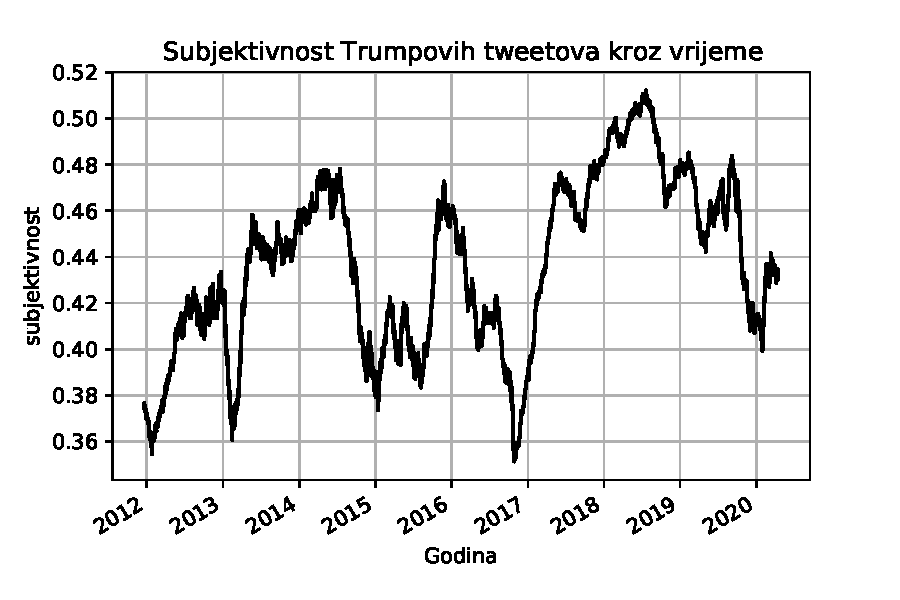
\includegraphics{"slike/subjektivnost.pdf"}
	\caption{Prikaz subjektivnosti Trumpovih \textit{tweetova} kroz zadnjih
	osam godina}
\end{figure}


\begin{figure}
	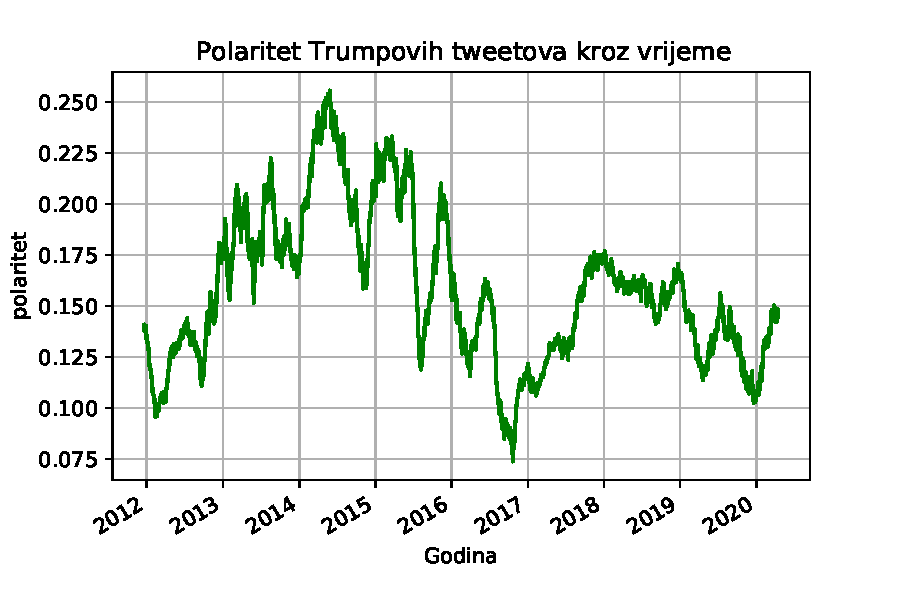
\includegraphics{"slike/polaritet.pdf"}
	\caption{Prikaz polariteta Trumpovih \textit{tweetova} kroz zadnjih
	osam godina}
\end{figure}

Iz danih dijagrama lako možemo povući zaključke -- unatoč tome što autor nije
upućen u društveno-politička zbivanja u SAD-u, lako je bilo pokazati da je za
vrijeme predsjedničke kampanje subjektivnost i polaritet \textit{tweetova}
drastično pao. Također se može zaključiti da polaritet nije pao u negativno,
već su \textit{tweetovi} postali \textit{manje pozivitivni}.

\chapter{Zaključak}

Ovaj projekt omogućio je svakom čitatelju upoznavanje s \texttt{TextBlobom} te
uvod u neurolingvističko programiranje. \texttt{TextBlob} je poprilično
jednostavan alat i stoga omogućuje početnicima u NLP-u strmiju krivulju učenja
koja je poprilično polegnuta kod korištenja biblioteke \texttt{NLTK}.

Takav pojednostavljeni pristup NLP-u je dobar za početak, no dosta se rano mogu
doživjeti ograničenja koja se mogu nadići tek malo snažnijim bibliotekama kao
što su \texttt{NLTK}, \texttt{Stanford CoreNLP}, \texttt{spaCy} i slični.

\nocite{*}
\bibliographystyle{plain}
\bibliography{lib}

Zbog prirode projekta citiralo se nije slijedno i prema dijelu u kojem je
nešto pročitano, već su ovi izvori poslužili kao izvori znanja. Stoga je autor
pisao svoje primjere temeljeno na ovim izvorima, a ništa se nije doslovno
preuzimalo.

\end{document}
